\documentclass[12pt,fleqn]{article}\usepackage{../common}
\begin{document}
Ders 5

Teori 

Bir kume $F$ kapalidir (closed), eger $F$ icindeki her yaklasiksal dizinin
1limiti yine $F$ icindeyse [ispat atlandi]. 

Tanim 

Vektoru uzayi $X$'ten reel (ya da kompleks) skalar uzayina yapilan
transformasyona $X$ uzerinde tanimli bir {\em fonksiyonel} denir. 

Dikkat fonksiyon degil, fonksiyonel. Fonksiyonelleri diger daha genel
transformasyonlardan ayirtetmek icin onlara notasyon olarak kucuk harfler
verilir, mesela $f,g$ gibi. 

Norm edilmis uzayda $f(x) = ||x||$ bir fonksiyonel ornegidir. Yani norm
operatorunun kendisi de bir fonksiyoneldir. Reel degerli fonksiyoneller
optimizasyon teorisi acisindan cok onemlidir normal olarak cunku
optimizasyonun amaci bir fonksiyoneli minimize (ya da maksimize) edecek bir
vektoru bulmaktir. 

$l_p$ ve $L_p$ Uzaylari 

Simdi derslerin geri kalaninda cok kullanacagimiz, faydali olacak bazi
klasik norm edilmis uzaylari gorelim. 

Tanim 

$0 < p < \infty$ olacak sekilde $p$ bir reel sayi olsun. $l_p$ uzayi $\{
\xi_1,\xi_2,...\xi_n\}$ 
skalar dizisidir, ki bu dizi su sarta uymalidir,

\[ \sum_{i=1}^{\infty} |\xi_i|^p < \infty \]

$p$ sayisi tanimlanan uzaya gore degisir, yani $l_3$ olabilir, bir digeri
$l_5$, vs. Bu uzayin normu nedir? Dikkat, ustteki bir norm degil, uzayi
tanimlamak icin kullandigimiz sartlardan biri. Norm, 

\[ ||x||_p = \bigg( \sum_{i=1}^\infty |\xi_i|^p \bigg)^{1/p}  \]

$l_\infty$ uzayi tum sinirli (bounded) dizileri icinde barindirir. $p =
\infty$ kullanilmasi
biraz garip gelebilir, $|\xi_i|$'in hem $\infty$ ile kati alinacak, hem de tum bu katlarin toplami 
sonsuzluktan kucuk olacak! 

$l_\infty$ icindeki bir oge $x = \{ \xi_i \}$'in normu 

\[ ||x||_\infty = \sup_i |\xi_i| \]

Banach Uzaylari 

Tanim

Bir norm edilmis uzayda $\{x_n\}$ dizisine Cauchy dizisi denmesinin sarti sudur:
Eger $m,n
\to \infty$ iken $||x_n - x_m|| \to 0$ dogru olmalidir; mesela verilen $\epsilon > 0$
icin oyle  bir $N$ olmalidir ki, her $n,m > N$ icin $||x_n - x_m|| < \epsilon$ dogru
olmalidir.

Bir norm edilmis uzayda her yaklasan dizi Cauchy dizisidir. Eger $x_n \to
x$ ise, 
o zaman 

\[ ||x_n - x_m|| = ||x_n -x +x -x_m|| \le 
||x_n - x|| + ||x-x_m|| \to 0
 \]

Fakat bu kuralin tersi her zaman dogru olmayabilir, yani her Cauchy dizisi
yaklasiksal olmayabilir. 

Icinde her Cauchy dizisinin yaklasiksal oldugu norm edilmis uzaylar
analizde ozellikle ilgi gorur, onemlidir, cunku bu tur uzaylarda
yaklasiksal dizileri bulmak / gostermek icin onlarin limitlerini bulmak
gerekmez (sadece Cauchy olduklarini gostermek yeter). Bu tur norm edilmis
uzaylara tam (complete) uzaylar denir.

Tanim

Norm edilmis uzay $X$ icindeki her Cauchy dizisinin $X$ icinde bir limiti
var ise, bu uzaya tam denir. Tam olan bir norm edilmis uzaya Banach Uzayi
ismi verilir. 

Uygulamalarda onumuze cikan problemleri Banach uzayina olan yansimasini /
orada da aynen isleyecek bir versiyonunu / esdegerini yaratmak icin oldukca
caba sarfederiz. Bu problemleri diger, cogunlukla tam olmayan, uzaylardan
cikartmak icin cok ugrasiriz, cunku optimizasyon problemlerinde Banach
uzaylarinin bir avantaji vardir; hedef fonsiyonunu maksimize edecek optimal
vektoru bulmak icin cogunlukla bir vektor dizisi yaratiriz, ve bu dizideki
her eleman bir oncekinden daha iyi olur, ve o zaman aradigimiz optimal
vektor otomatik olarak bu dizinin limiti olacaktir. Bu teknigin ise
yaramasi icin limiti hesaplayamiyor olsak bile, bu dizinin yaklastigini bir
sekilde bilmemiz gerekir / bunu bize gosterecek bir test
gerekir. Yaklasiksallik icin Cauchy kriteri iste bunu saglar, temel
aldigimiz uzay tam ise, Cauchy dizisinin yaklasacagindan emin olabiliriz.

Simdi tam olmayan bir norm edilmis uzay gorelim. 

Ornek

$X$ uzayi $[0,1]$ uzerinde tanimli tum surekli fonsiyonlar olsun, ve norm
$\|x\| = \int_{0}^{1} |x(t)|dt$. $X$'in tam olmadigini ispat icin $X$ icinde soyle bir 
dizi yaratacagiz, 



\[ 
 x_n(t) =
\left\{ \begin{array}{ll}
0 &  0 \le t \le \frac{1}{2} - \frac{1}{n} \\ \\
nt-\frac{n}{2} + 1 &  \frac{1}{2} - \frac{1}{n} \le t \le \frac{1}{2} \\ \\
1 & t \ge \frac{1}{2}
\end{array} \right.
 \]

Bu dizinin her elemani bir surekli fonsiyondur ve bu yuzden $X$'in bir
uyesidir. 

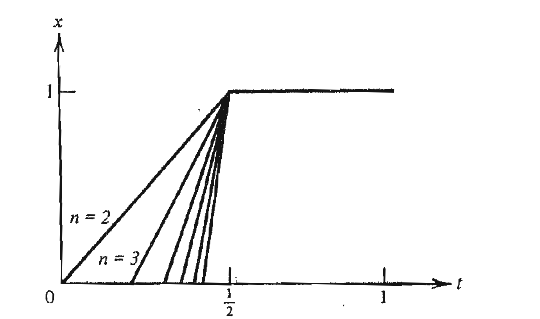
\includegraphics[height=6cm]{5_1.png}

Bu dizi Cauchy midir? $||x_n - x_m||$'i hesaplayalim ve $n,m \to \infty$
iken ne oluyor ona bakalim. Aslinda hesap icin entegralleri cebirsel olarak
hesaplamaya gerek yok, entegral $f$'in altindaki alani hesapladigina gore,
gorsel olarak dusunebiliriz. Ustteki grafikte gordugumuz gibi her $n$ yeni
bir fonsiyon yaratir. Fakat $n,m$ sonsuza gittikce ikisi de basamak (step)
fonsiyonu olmaya yaklasacaktir, ve farklarinin normu $||x_n - x_m||$ sifira
yaklasacaktir. Alan farki icin tam formul

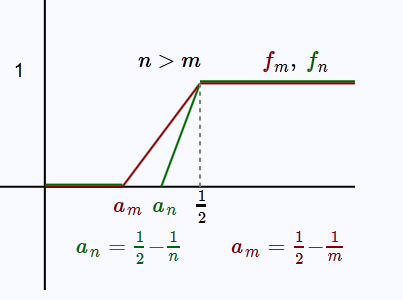
\includegraphics[height=6cm]{5_2.png}

\[ 
\frac{1}{2} \cdot 1 \cdot (\frac{ 1}{2}-a_m) - 
\frac{1}{2} \cdot 1 \cdot (\frac{ 1}{2}-a_n) =
\frac{ 1}{2}\frac{ 1}{m} - 
\frac{ 1}{2}\frac{ 1}{n} 
 \]

Yani

\[ ||x_n - x_m|| = \frac{ 1}{2}|1/n - 1/m| \]

Grafikte sadece pozitif kisim gozukuyor cunku unutmayalim, $t$ degerleri
$[0,1]$ arasinda geliyor, ve formuldeki tum parcalar buna gore pozitif
degerler uretiyorlar. 

Teori 

Bir Cauchy dizisi sinirlidir

Ispat

$\{x_n\}$ bir Cauchy dizisi diyelim, ve $N$ oyle bir tam sayi olsun ki $n >
N$ 
icin $||x_n - x_N|| < 1$ dogru olacak. $n > N$ icin

\[ ||x_n|| = ||x_n - x_N + x_N || \le ||x_N|| + ||x_n - x_N|| < ||x_N|| + 1 \]

\[ \square \]

Ornek

$C[0,1]$ bir Banach uzayidir. Daha once bu uzayin tam oldugunu
soylemistik. $C[0,1]$'in tam oldugunu ispatlamak icin $C[0,1]$ icindeki her
Cauchy dizisinin bir limiti oldugunu gostermek yeterlidir. 

Diyelim ki $\{x_n\}$ $C[0,1]$ icinde bir Caucy dizisi. Her sabit $t \in
[0,1]$ 
icin $|x_n(t) - x_m(t)| \le ||x_n - x_m|| \to 0$, o zaman  $\{x_n(t)\}$
reel sayilardan olusan bir Cauchy dizisidir. Bu dizi dogal olarak reel
sayilar uzayi $\mathbb{R}$'dedir, ve $\mathbb{R}$'nin tam oldugunu
biliyoruz. O zaman bu dizinin yaklastigi bir $x(t)$ her zaman olacaktir,
yani $x_n(t) \to x(t)$. Bunun sonucu olarak $x_n$ fonksiyonlari da $x$'e
yaklasmalidir. 

Genel olarak tarif etmek gerekirse, $x_n$ dizisini $\mathbb{R}$'deki bir
baska dizi $\{x_n(t)\}$'ye indirgiyoruz, yani yansimasini yaratiyoruz,
sectigimiz tek bir $t$ uzerinden. Uzayi degistirmemizin avantaji su,
$\mathbb{R}$'nin tam oldugunu biliyoruz. O zaman oraya indirgedigimiz
Cauchy dizisinin o uzayda muhakkak bir limiti olmalidir. Simdi,
$\mathbb{R}$'den filmi geriye sariyoruz, her $t$ icin ``yukari cikarken''
elimizdeki limitleri toparliyoruz, ve $x_n$ seviyesine getiriyoruz. Bunu
tum $t$'ler icin yapabildigimize gore, o zaman tum $x_n$'nin de bir limiti
olmalidir.






\end{document}
